\documentclass[pdftex,francais]{beamer}

% Copyright 2004 by Till Tantau <tantau@users.sourceforge.net>.
%
% This file can be redistributed and/or modified under
% the terms of the GNU Public License, version 2.

%% \ifx\themename\undefined
%%   \def\themename{default}
%% \fi

\usetheme{lama}
%\usetheme{Madrid}
%\usecolortheme{crane}

\usepackage{multirow}
\usepackage[latin1]{inputenc}           %%%  
\usepackage[T1]{fontenc}                %%%
\usepackage[francais]{babel}            %%%

\usepackage{multimedia}
\usepackage{hyperref}
\usepackage{tikz}
\usepackage{listings}

%\newtheorem{theorem}{Théorème}

%\setbeamercovered{transparent}

\title[Digital surfaces in DGtal]{Digital surfaces in DGtal\\
     Topology module (since 0.5)
}

\author[J.-O. Lachaud]{Jacques-Olivier Lachaud}

\date{DGtal Meeting, june 2012}


\graphicspath{{Figures/},{Images/},{Graphs/}}

%%% \AtBeginSection[]
%%% {
%%%   \begin{frame}<beamer>
%%%     \frametitle{Plan}
%%%     \tableofcontents[currentsection] %,currentsubsection]
%%%   \end{frame}
%%% }


\renewcommand{\vec}[1]{\mathbf{#1}}

% space of the real numbers
\newcommand{\R}{\ensuremath{\mathbb{R}}}
% space of the integer numbers
\newcommand{\Z}{\ensuremath{\mathbb{Z}}}
% Digitization process of step h (1)
\newcommand{\Dig}[1]{\ensuremath{\mathrm{Dig}_{#1}}}
% Family of shape
\newcommand{\SF}[0]{\ensuremath{\mathbb{F}}}
% Topological boundary of X (1).
\newcommand{\TB}[1]{\ensuremath{\partial #1}}
% Discrete geometric estimator of G (1)
\newcommand{\DGE}[1]{\ensuremath{E_{#1}}}
% Reference shape of digital object O (1) with grid step $h$ (2).
\newcommand{\RS}[2]{\ensuremath{R_{#1,#2}}}

% Digital contour.
\newcommand{\DC}{\ensuremath{C}}
% Continuous contour.
\newcommand{\CC}{\ensuremath{\mathcal{C}}}
% A point indexed by i (1) on the digital contour.
\newcommand{\PT}[1]{\ensuremath{\DC_{#1}}}
% A sequence of points indexed by i (1) on the digital contour.
\newcommand{\PTS}[2]{\ensuremath{\DC_{#1,#2}}}
% Predicate stating that the digital curve is a segment between indices 1 and 2
\newcommand{\SPRED}[2]{\ensuremath{S(#1,#2)}}
% ET logique
\newcommand{\AND}[0]{\ensuremath{\wedge}}
% OU logique
\newcommand{\OR}[0]{\ensuremath{\vee}}

% Tangent direction mapping of curve C (1)
\newcommand{\TGT}[1]{\ensuremath{\theta_{#1}}}
% Integral of squared curvature of curve C (1)
\newcommand{\ISC}[1]{\ensuremath{J[#1]}}
% Smallest possible tangent direction at constraint l (1)
\newcommand{\MinTD}[1]{\ensuremath{a_{#1}}}
% Largest possible tangent direction at constraint l (1)
\newcommand{\MaxTD}[1]{\ensuremath{b_{#1}}}
% Unknown tangent direction at constraint l (1)
\newcommand{\UnkTD}[1]{\ensuremath{t_{#1}}}

% ideal multiscale criterion
\newcommand{\IMSC}[2]{\ensuremath{\mu_{#1}(#2)}}
% multiscale profile
\newcommand{\MSP}[2]{\ensuremath{\mathcal{P}_{#1}(#2)}}
% threshold flat/curve
\newcommand{\CThreshold}[0]{\ensuremath{t_{f/c}}}
% threshold noise
\newcommand{\NThreshold}[0]{\ensuremath{t_{m}}}
% noise level
\newcommand{\NL}[0]{\ensuremath{\nu}}
% slope linear regression 
\newcommand{\SLR}[2]{\ensuremath{\theta_{#1}}}





% Pencil of maximal segments around a point.
\newcommand{\PE}[1]{\ensuremath{{\mathcal P}(#1)}}
% Tangent orientation of the maximal segment.
\newcommand{\TO}[1]{\ensuremath{\theta_#1}}
% lambda function for interpolation.
\newcommand{\LF}{\ensuremath{\lambda}}
% \lambda-MS tangent orientation.
\newcommand{\LTO}[1]{\ensuremath{\hat{\theta}(#1)}}
% \lambda-MS tangent orientation variation.
\newcommand{\LTOP}[1]{\ensuremath{\hat{\theta}'(#1)}}

%\definecolor{rougeSW_}{rgb}{0.968627,0.011765,0.015686}
\definecolor{darkgreen}{rgb}{0.0,0.6,0.0}
\definecolor{lightblue}{rgb}{0.5,0.5,1.0}
\definecolor{magenta}{rgb}{1.0,0.0,1.0}
\newcommand{\alertred}[1]{{\color{red}#1}}
\newcommand{\Cb}[1]{{\color{blue}#1}}
\newcommand{\Cdg}[1]{{\color{darkgreen}#1}}
\newcommand{\textmagenta}[1]{{\color{magenta}#1}}
\newcommand{\Implies}{{\ensuremath{\Rightarrow}}}

\newcommand{\Refs}[1]{{\color{lightblue}#1}}
\newcommand{\Cite}[1]{\Refs{[#1]}}
\newcommand{\Etal}{{\em et al.}}
\newtheorem{remark}{Remarque}
% Digitization process of step h (1)
\newcommand{\DigGh}[2]{\ensuremath{\mathrm{Dig}_{#2}(#1)}}
\newcommand{\BigT}{\ensuremath{\Theta}}
\newcommand{\BigO}{\ensuremath{O}}

\newcommand{\TAN}[0]{\ensuremath{\theta}}
% Position estimator
\newcommand{\EPOS}[0]{\ensuremath{\hat{{x}}}}
% Convexity Position estimator 
\newcommand{\ECONVPOS}[0]{\ensuremath{\hat{x}^\mathrm{conv}}}
% tangent estimator base MS.
\newcommand{\ETANMS}[0]{\ensuremath{\hat{\TAN}^{\text{MS}}}}
% tangent estimator base arete du CDP.
\newcommand{\ETANEDGE}[0]{\ensuremath{\hat{\TAN}^{\text{conv}}}}
% estimateur de longueur elementaire d'un surfel (1) sur le bord discretise de X(2) de pas h(3).

\newcommand{\Class}[1]{\alert{\texttt{#1}}}
\newcommand{\Concept}[1]{\texttt{\color{magenta}#1}}
\newcommand{\Method}[1]{\texttt{\color{lightblue}#1}}


\setbeamercolor{qcolorb}{fg={blue!20!black},bg={blue!15!white}}
\setbeamercolor{qcolorub}{fg={blue!10!black},bg={blue!30!white}}
\setbeamercolor{qcolorlb}{fg={blue!20!black},bg={blue!8!white}}
\setbeamercolor{qcolorulb}{fg={blue!10!black},bg={blue!40!white}}
\setbeamercolor{qcolorg}{fg={green!20!black},bg={green!15!white}}
\setbeamercolor{qcolorug}{fg={green!10!black},bg={green!30!white}}
\setbeamercolor{qcolorlg}{fg={green!20!black},bg={green!8!white}}
\setbeamercolor{qcolorulg}{fg={green!10!black},bg={green!40!white}}
\setbeamercolor{qcolorr}{fg={red!20!black},bg={red!15!white}}
\setbeamercolor{qcolorur}{fg={red!10!black},bg={red!30!white}}
\setbeamercolor{qcolorlr}{fg={red!20!black},bg={red!8!white}}
\setbeamercolor{qcolorulr}{fg={red!10!black},bg={red!40!white}}
\newenvironment{myblockbluish}[2]%
	       {\begin{beamerboxesrounded}[lower=qcolorb,upper=qcolorub,width=#1,shadow=true]{#2}}{\end{beamerboxesrounded}}
\newenvironment{myblocklbluish}[2]%
	       {\begin{beamerboxesrounded}[lower=qcolorlb,upper=qcolorulb,width=#1,shadow=true]{#2}}{\end{beamerboxesrounded}}
\newenvironment{myblockgreenish}[2]%
	       {\begin{beamerboxesrounded}[lower=qcolorg,upper=qcolorug,width=#1,shadow=true]{#2}}{\end{beamerboxesrounded}}
\newenvironment{myblocklgreenish}[2]%
	       {\begin{beamerboxesrounded}[lower=qcolorlg,upper=qcolorulg,width=#1,shadow=true]{#2}}{\end{beamerboxesrounded}}
\newenvironment{myblockredish}[2]%
	       {\begin{beamerboxesrounded}[lower=qcolorr,upper=qcolorur,width=#1
,shadow=true]{#2}}{\end{beamerboxesrounded}}
\newenvironment{myblocklredish}[2]%
	       {\begin{beamerboxesrounded}[lower=qcolorlr,upper=qcolorulr,width=#1,shadow=true]{#2}}{\end{beamerboxesrounded}}

%%%%%%%%%%%%%%%%%%%%%%%%%%%%%%%%%%%%%%%%%%%%%%%%%%%%%%%%%%%%%%%%%%%%%%%%%%%%%%%
%%%%%%%%%%%%%%%%%%%%%%%%%%%%%%%%%%%%%%%%%%%%%%%%%%%%%%%%%%%%%%%%%%%%%%%%%%%%%%%
%%%%%%%%%%%%%%%%%%%%%%%%%%%%%%%%%%%%%%%%%%%%%%%%%%%%%%%%%%%%%%%%%%%%%%%%%%%%%%%
\begin{document}

\newlength{\unquart}
\setlength{\unquart}{0.21\textwidth}

%------------------------------------------------------------------------------
\begin{frame}
  \titlepage
\end{frame}
%------------------------------------------------------------------------------

\section{Introduction}

%------------------------------------------------------------------------------
\begin{frame}%[allowframebreaks]
  \frametitle{Available in DGtal 0.5}
  
  \begin{enumerate}
  \item classical digital topology
    \begin{itemize}
    \item Arbitrary adjacencies in $\Z^n$, but also in subdomains
    \item Digital topology = couple of adjacencies (Rosenfeld)
    \item Object = Topology + Set
    \item Operations: neighborhoods, border, connectedness and connected
      components, decomposition into digital layers, simple points
    \end{itemize}

    \only<1>{
      \begin{tabular}{cc}
        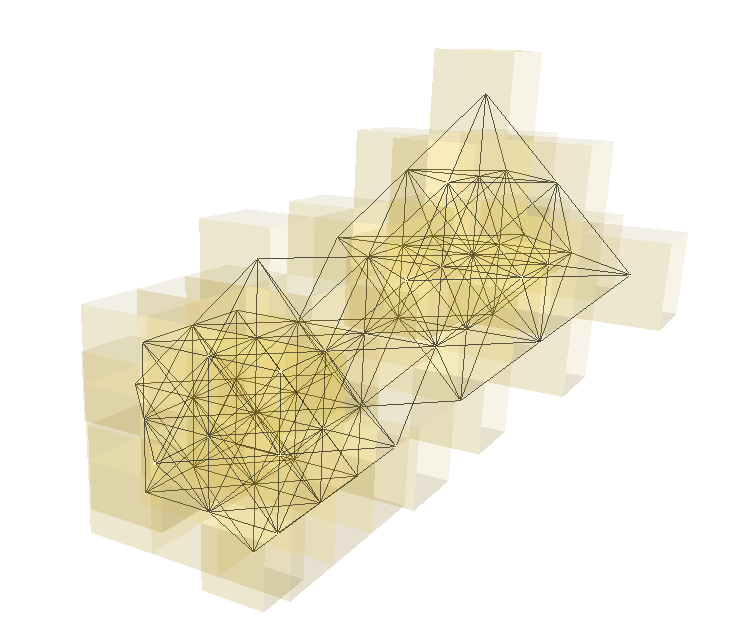
\includegraphics[width=0.4\textwidth]{object-3d-18-6} & 
        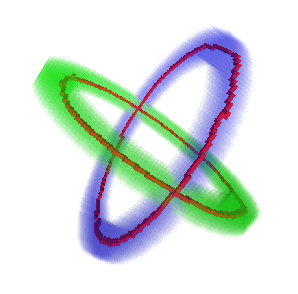
\includegraphics[width=0.3\textwidth]{thinning-3d} \\
        Adjacencies &
        thinning in (6,26) \\
      \end{tabular}
    }

    \only<2-3>{
    \item cubical cellular topology
      \begin{itemize}
      \item cells, adjacent and incident cells, faces and cofaces
      \item signed cells, signed incidence, 
      \end{itemize}
    }
    \only<3>{
    \item digital surface topology
      \begin{itemize}
      \item surfels, surfel adjacency, surfel neighborhood
      \item surface tracking (normal, fast), contour tracking in $n$D
      \end{itemize}
    }
  \end{enumerate}
\end{frame}
%------------------------------------------------------------------------------


%------------------------------------------------------------------------------
\begin{frame}[squeeze]%[allowframebreaks]
  \frametitle{Package description}

  \begin{myblocklbluish}{\textwidth}{Should contain}
    \begin{itemize}
      \small
    \item classical digital topology {\em à la} Rosenfeld
    \item cartesian cellular topology
    \item digital surface topology {\em à la} Herman
    \item must be the base block of geometric algorithms
    \end{itemize}
  \end{myblocklbluish}
  \begin{myblocklgreenish}{\textwidth}{Examples}
    \begin{itemize}
      \small
    \item adjacencies, connected components, simple points, thinning
    \item cells, boundary operators, incidence, opening, closing
    \item contours, surfel adjacency, surface tracking
    \item topological invariants
    \end{itemize}
  \end{myblocklgreenish}
  \begin{myblocklredish}{\textwidth}{Location}
    \begin{itemize}
      \small
    \item \texttt{\{DGtal\}/src/DGtal/topology}
    \item \texttt{\{DGtal\}/src/DGtal/helpers}
    \item \texttt{\{DGtal\}/tests/topology}
    \end{itemize}
  \end{myblocklredish}

\end{frame}
%------------------------------------------------------------------------------


\end{document}
